\begin{enumerate}
\item % (a)

Our implementation for the Fresnel term is found in Listing \ref{lst:5-5-a}.

\begin{lstlisting}[caption={Function to compute the Fresnel term},label={lst:5-5-a}]
float compute_fresnel(const Vector3f& v, float eta, float k) {
    float sin = Frame::sinTheta(v);
    float cos = Frame::cosTheta(v);
    float tan = Frame::tanTheta(v);
    float sin2 = sin * sin;
    float cos2 = cos * cos;
    float tan2 = tan * tan;

    float eta2 = eta * eta;
    float k2 = k * k;
    float eta2k2sin2 = eta2 - k2 - sin2;

    float root = std::sqrt(eta2k2sin2 * eta2k2sin2 + 4 * eta2 * k2);
    float a2 = 0.5 * (root + eta2k2sin2);
    float b2 = 0.5 * (root - eta2k2sin2);
    float a = std::sqrt(a2);

    float R_s = (a2 + b2 - 2 * a * cos + cos2) /
                (a2 + b2 + 2 * a * cos + cos2);

    float R_p = R_s * (a2 + b2 - 2 * a * sin * tan + sin2 * tan2) /
                      (a2 + b2 + 2 * a * sin * tan + sin2 * tan2);

    return 0.5f * (R_s + R_p);
}
\end{lstlisting}

\item % (b)

Our implementation for the conductor BSDF model is found in Listing \ref{lst:5-5-b}.

\begin{lstlisting}[caption={Our implementation for the conductor BSDF model},label={lst:5-5-b}]
#include "nori/common.h"
#include <cmath>
#include <cstdlib>
#include <nori/bsdf.h>
#include <nori/texture.h>
#include <nori/frame.h>
#include <nori/warp.h>

NORI_NAMESPACE_BEGIN

/**
 * \brief Conductor BRDF model
 */
class Conductor : public BSDF {
public:
    Conductor(const PropertyList &propList) {
        m_eta = propList.getColor("eta");
        m_k = propList.getColor("k");
    }

    /**
     * \brief Evaluate the BSDF for a pair of directions and measure
     * specified in \code bRec
     *
     * \param bRec
     *     A record with detailed information on the BSDF query
     * \return
     *     The BSDF value, evaluated for each color channel
     */
    Color3f eval(const BSDFQueryRecord &bRec) const override {
        return {0.0f};
    }

    /**
     * \brief Compute the probability of sampling \c bRec.wo
     * (conditioned on \c bRec.wi).
     *
     * This method provides access to the probability density that
     * is realized by the \ref sample() method.
     *
     * \param bRec
     *     A record with detailed information on the BSDF query
     *
     * \return
     *     A probability density value expressed with respect
     *     to the specified measure
     */
    float pdf(const BSDFQueryRecord &bRec) const override {
        return 0.0f;
    }

    /**
     * \brief Sample the BSDF and return the importance weight (i.e. the
     * value of the BSDF * cos(theta_o) divided by the probability density
     * of the sample with respect to solid angles).
     *
     * \param bRec    A BSDF query record
     * \param sample  A uniformly distributed sample on \f$[0,1]^2\f$
     *
     * \return The BSDF value divided by the probability density of the sample,
     *         multiplied by the cosine factor associated with the outgoing direction.
     *         A zero value means that sampling failed.
     */
    Color3f sample(BSDFQueryRecord &bRec, const Point2f &sample) const override {
        bRec.wo = Vector3f{
            -bRec.wi.x(),
            -bRec.wi.y(),
            bRec.wi.z(),
        };

        Color3f F_r(
            compute_fresnel(bRec.wo, m_eta.r(), m_k.r()),
            compute_fresnel(bRec.wo, m_eta.g(), m_k.g()),
            compute_fresnel(bRec.wo, m_eta.b(), m_k.b())
        );
        bRec.measure = EDiscrete;

        float costheta = std::abs(Frame::cosTheta(bRec.wo));
        return {
            F_r.r() / costheta,
            F_r.g() / costheta,
            F_r.b() / costheta,
        };
    }

    /// Return a human-readable summary
    std::string toString() const override {
        return tfm::format(
                    "Conductor[\n"
                    "  eta = %s,\n"
                    "  k = %s,\n"
                    "]", m_eta.toString(), m_k.toString());
    }

    EClassType getClassType() const  override { return EBSDF; }
private:
    Color3f m_eta;
    Color3f m_k;
};

NORI_REGISTER_CLASS(Conductor, "conductor");
NORI_NAMESPACE_END

\end{lstlisting}

\item % (c)

Our implementation for the dielectric BSDF model is found in Listing \ref{lst:5-5-c}.

\begin{lstlisting}[caption={Our implementation for the dielectric BSDF model},label={lst:5-5-c}]
#include <nori/bsdf.h>
#include <nori/texture.h>
#include <nori/frame.h>
#include <nori/warp.h>

NORI_NAMESPACE_BEGIN

/**
 * \brief Dielectric BRDF model
 */
class Dielectric : public BSDF {
public:
    Dielectric(const PropertyList &propList) {
        m_extIOR = propList.getFloat("extIOR");
        m_intIOR = propList.getFloat("intIOR");
    }

    /**
     * \brief Evaluate the BSDF for a pair of directions and measure
     * specified in \code bRec
     *
     * \param bRec
     *     A record with detailed information on the BSDF query
     * \return
     *     The BSDF value, evaluated for each color channel
     */
    Color3f eval(const BSDFQueryRecord &bRec) const override {
        return {0.0f};
    }

    /**
     * \brief Compute the probability of sampling \c bRec.wo
     * (conditioned on \c bRec.wi).
     *
     * This method provides access to the probability density that
     * is realized by the \ref sample() method.
     *
     * \param bRec
     *     A record with detailed information on the BSDF query
     *
     * \return
     *     A probability density value expressed with respect
     *     to the specified measure
     */
    float pdf(const BSDFQueryRecord &bRec) const override {
        return 0.0f;
    }

    /**
     * \brief Sample the BSDF and return the importance weight (i.e. the
     * value of the BSDF * cos(theta_o) divided by the probability density
     * of the sample with respect to solid angles).
     *
     * \param bRec    A BSDF query record
     * \param sample  A uniformly distributed sample on \f$[0,1]^2\f$
     *
     * \return The BSDF value divided by the probability density of the sample,
     *         multiplied by the cosine factor associated with the outgoing direction.
     *         A zero value means that sampling failed.
     */
    Color3f sample(BSDFQueryRecord &bRec, const Point2f &sample) const override {
        bRec.wi.normalize();
        bRec.measure = EDiscrete;

        // determine the incident and transmitted IOR
        float etaI = m_extIOR;
        float etaT = m_intIOR;
        float sgn = 1.0;

        if (bRec.wi.z() < 0.0f) {
            std::swap(etaI, etaT);
            sgn = -1.0;
        }

        // relative IOR
        float eta = etaI / etaT;

        // fresnel reflectance
        float cosThetaI = std::abs(bRec.wi.z());
        float F_r = fresnelDielectric(cosThetaI, etaI, etaT);

        // reflection direction
        Vector3f wr = Vector3f{
            -bRec.wi.x(),
            -bRec.wi.y(),
            bRec.wi.z(),
        };

        // check for total internal reflection
        float sinThetaT2 = eta * eta * (1.0f - cosThetaI * cosThetaI);

        if (sinThetaT2 >= 1.0) {
            bRec.wo = wr;
            return {1.0f};
        }

        // choose relfection or refraction
        if (F_r > sample.x()) {
            // reflection
            bRec.wo = wr;
            return {1.0};
        } else {
            // refraction
            float cosThetaT = std::sqrt(1.0f - sinThetaT2);

            bRec.wo = Vector3f{
                -eta * bRec.wi.x(),
                -eta * bRec.wi.y(),
                -sgn * cosThetaT,
            };

            bRec.eta = etaT / etaI;
            return {eta * eta};
        }
    }

    /// Return a human-readable summary
    std::string toString() const override {
        return tfm::format(
                    "Dielectric[\n"
                    "  extIOR = %f,\n"
                    "  intIOR = %f,\n"
                    "]", m_extIOR, m_intIOR);
    }

    EClassType getClassType() const  override { return EBSDF; }

    void computeReflectance(float n, float k, float& R_s, float& R_p) {
    }
private:
    float m_extIOR;
    float m_intIOR;
};

NORI_REGISTER_CLASS(Dielectric, "dielectric");
NORI_NAMESPACE_END

\end{lstlisting}

\item % (d)

Our code for the conductor does not seem correct. It is way too bright in comparison to the reference image. Especially close surfaces, which are parallel to each other, appear to generate light. This is seen in the comparison Figure \ref{fig:ingots-compare}, which has a green tint. This probably results from the values of each pixel or our result being significantly higher than the reference. We couldn't fiure out the correct code and decided to turn it in anyway.

The dialectric translucent ingot appears correct however. The parts of it that are not bent into a conducting ingot are quite dark in the comparison, suggesting that the returned color is correct.

\begin{figure}[H]
    \centering
    \begin{minipage}{0.32\textwidth}
        \centering
        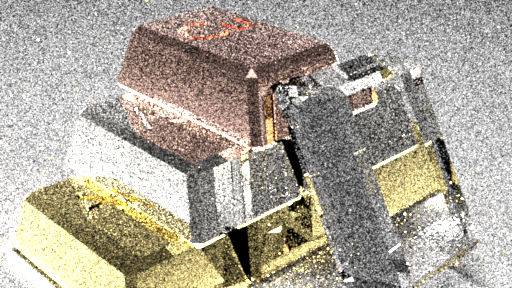
\includegraphics[width=\linewidth]{pictures/ingots-bsdfpath.png}
        \caption{Our result of the ingots scene}
        \label{fig:ingots-result}
    \end{minipage}
    \hfill
    \begin{minipage}{0.32\textwidth}
        \centering
        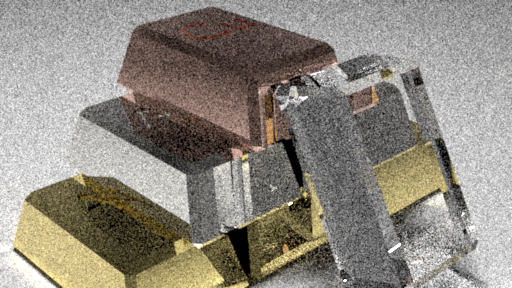
\includegraphics[width=\linewidth]{pictures/ingots-bsdfpath-512spp-ref.png}
        \caption{The reference image of the ingots scene}
        \label{fig:ingots-reference}
    \end{minipage}
    \hfill
    \begin{minipage}{0.32\textwidth}
        \centering
        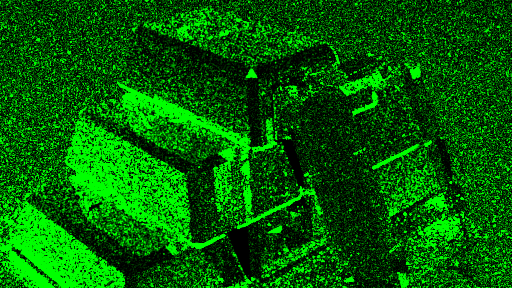
\includegraphics[width=\linewidth]{pictures/ingots-bsdfpath-compare.png}
        \caption{Comparison between our result vs reference}
        \label{fig:ingots-compare}
    \end{minipage}
\end{figure}

\end{enumerate}